%-----------------------------------------------
% Assignment 2: Data Handling and Visualization
%-----------------------------------------------
\refstepcounter{section}
\addlabcontentsline{Assignment \thesection: Data Handling and Visualization}{11-09-2025}{\thepage}
\section*{\centering Assignment \thesection: Data Handling and Visualization}

\noindent \textbf{Objective:} To explore real-world datasets using NumPy, Pandas, Matplotlib, and
Seaborn, focusing on statistical insights, cleaning, and visualization for
better decision-making.
\vspace{-1em}

%-----------------------------------------------
% Task 1
%-----------------------------------------------
\subsection{Task 1: Weather Data Analysis (NumPy Operations)}
\vspace{-0.1em}
\subsubsection*{Code Implementation}
% \vspace{-1em}
\begin{lstlisting}[style=pythonStyle, caption={}]
# ------------------------------------------
# Task 1: Weather Data Analysis (NumPy)
# ------------------------------------------

import numpy as np  


temperatures = np.random.randint(20, 41, size=30)  
print("Daily Temperatures (°C):\n", temperatures)


mean_temp = np.mean(temperatures)
median_temp = np.median(temperatures)
std_temp = np.std(temperatures)

print("\n Statistical Insights:")
print("Mean Temperature:", mean_temp)
print("Median Temperature:", median_temp)
print("Standard Deviation:", std_temp)


normalized_temps = (temperatures - np.min(temperatures)) / (np.max(temperatures) - np.min(temperatures))
print("\nNormalized Temperatures (0-1):\n", normalized_temps)


temp_matrix = temperatures.reshape(5, 6)
print("\nTemperature Matrix (5 weeks x 6 days):\n", temp_matrix)


transposed_matrix = temp_matrix.T
print("\nTransposed Matrix:\n", transposed_matrix)


rainfall = np.random.randint(0, 101, size=(5, 6))
print("\nRainfall Matrix (mm):\n", rainfall)


addition = temp_matrix + rainfall
print("\nMatrix Addition (Temp + Rainfall):\n", addition)


multiplication = temp_matrix * rainfall
print("\nMatrix Multiplication (Temp * Rainfall):\n", multiplication)
    
\end{lstlisting}

\vspace{1em} 
\subsubsection*{Output}
\begin{Numbox}
    \begin{verbatim}
Daily Temperatures (deg C):

 [28 36 30 31 34 31 37 31 34 25 23 29 37 23 29 24 25 39 37 35 24 28 25 30
 23 24 27 20 38 39]

Statistical Insights:

Mean Temperature: 29.866666666666667

Median Temperature: 29.5
    Daily Temperatures (deg C):

 [28 36 30 31 34 31 37 31 34 25 23 29 37 23 29 24 25 39 37 35 24 28 25 30
 23 24 27 20 38 39]

 Statistical Insights:

 Mean Temperature: 29.866666666666667

 Median Temperature: 29.5

 Standard Deviation: 5.530119548637464

 Normalized Temperatures (0-1):

 [0.42105263 0.84210526 0.52631579 0.57894737 0.73684211 0.57894737
 0.89473684 0.57894737 0.73684211 0.26315789 0.15789474 0.47368421
 0.89473684 0.15789474 0.47368421 0.21052632 0.26315789 1.
 0.89473684 0.78947368 0.21052632 0.42105263 0.26315789 0.52631579
 0.15789474 0.21052632 0.36842105 0.         0.94736842 1.        ]

Temperature Matrix (5 weeks x 6 days):
 [[28 36 30 31 34 31]
 [37 31 34 25 23 29]
 [37 23 29 24 25 39]
 [37 35 24 28 25 30]
 [23 24 27 20 38 39]]

Transposed Matrix:
[[28 37 37 37 23]
[36 31 23 35 24]
[30 34 29 24 27]
[31 25 24 28 20]
[34 23 25 25 38]
[31 29 39 30 39]]

Rainfall Matrix (mm):
[[92 82 71 63  5 67]
[59 67 18 36 32 67]
[24 56 60 28 96 93]
[27 42 87 25 53 69]
[22 97 87 74 44 16]]

Matrix Addition (Temp + Rainfall):
[[120 118 101  94  39  98]
[ 96  98  52  61  55  96]
[ 61  79  89  52 121 132]
[ 64  77 111  53  78  99]
[ 45 121 114  94  82  55]]

Matrix Multiplication (Temp * Rainfall):
[[2576 2952 2130 1953  170 2077]
[2183 2077  612  900  736 1943]
[ 888 1288 1740  672 2400 3627]
[ 999 1470 2088  700 1325 2070]
[ 506 2328 2349 1480 1672  624]]

\end{verbatim}
\end{Numbox}

%-----------------------------------------------
% Task 2
%-----------------------------------------------
\subsection{Task 2: Student Records Management (Pandas Basics)}
\vspace{-0.1em}
\subsubsection*{Code Implementation}
% \vspace{-1em}
\begin{lstlisting}[style=pythonStyle, caption={Load the file StudentsPerformance.csv.}]
import pandas as pd  

data = pd.read_csv("StudentsPerformance.csv")

print("Preview of Dataset:")
print(data.head())
    
\end{lstlisting}

\vspace{1em} 
% \subsubsection*{Output}
\begin{outputbox}
\begin{verbatim}
Preview of Dataset:
   gender race/ethnicity parental level of education         lunch  \
0  female        group B           bachelor's degree      standard   
1  female        group C                some college      standard   
2  female        group B             master's degree      standard   
3    male        group A          associate's degree  free/reduced   
4    male        group C                some college      standard   

  test preparation course  math score  reading score  writing score  
0                    none          72             72             74  
1               completed          69             90             88  
2                    none          90             95             93  
3                    none          47             57             44  
4                    none          76             78             75  

\end{verbatim}

\end{outputbox}

\begin{lstlisting}[style=pythonStyle, caption={Display dataset summary (info(), describe()).}]
print("Dataset Info:")
print(data.info())
print("\nDataset Description:")
print(data.describe(include="all"))
    
\end{lstlisting}

\vspace{1em} 
% \subsubsection*{Output}
\begin{outputbox}
\begin{verbatim}
    Dataset Info:
<class 'pandas.core.frame.DataFrame'>
RangeIndex: 1000 entries, 0 to 999
Data columns (total 8 columns):
 #   Column                       Non-Null Count  Dtype 
---  ------                       --------------  ----- 
 0   gender                       1000 non-null   object
 1   race/ethnicity               1000 non-null   object
 2   parental level of education  1000 non-null   object
 3   lunch                        1000 non-null   object
 4   test preparation course      1000 non-null   object
 5   math score                   1000 non-null   int64 
 6   reading score                1000 non-null   int64 
 7   writing score                1000 non-null   int64 
dtypes: int64(3), object(5)
memory usage: 62.6+ KB
None

Dataset Description:
        gender race/ethnicity parental level of education     lunch  \
count     1000           1000                        1000      1000   
unique       2              5                           6         2   
top     female        group C                some college  standard   
freq       518            319                         226       645   
mean       NaN            NaN                         NaN       NaN   
std        NaN            NaN                         NaN       NaN   
min        NaN            NaN                         NaN       NaN   
25%        NaN            NaN                         NaN       NaN   
50%        NaN            NaN                         NaN       NaN   
75%        NaN            NaN                         NaN       NaN   
max        NaN            NaN                         NaN       NaN   

       test preparation course  math score  reading score  writing score  
count                     1000  1000.00000    1000.000000    1000.000000  
unique                       2         NaN            NaN            NaN  
top                       none         NaN            NaN            NaN  
freq                       642         NaN            NaN            NaN  
mean                       NaN    66.08900      69.169000      68.054000  
std                        NaN    15.16308      14.600192      15.195657  
min                        NaN     0.00000      17.000000      10.000000  
25%                        NaN    57.00000      59.000000      57.750000  
50%                        NaN    66.00000      70.000000      69.000000  
75%                        NaN    77.00000      79.000000      79.000000  
max                        NaN   100.00000     100.000000     100.000000 

    
\end{verbatim}

\end{outputbox}

\begin{lstlisting}[style=pythonStyle, caption={Group students by gender and compute the average math score.}]
avg_math_by_gender = data.groupby("gender")["math score"].mean()
print("\nAverage Math Score by Gender:\n", avg_math_by_gender)
    
\end{lstlisting}

\vspace{1em} 
% \subsubsection*{Output}
\begin{outputbox}
\begin{verbatim}
Average Math Score by Gender:
 gender
female    63.633205
male      68.728216
Name: math score, dtype: float64
    
\end{verbatim}

\end{outputbox}

\begin{lstlisting}[style=pythonStyle, caption={Identify which parental education level leads to the highest average
reading score.}]
avg_reading_by_parent = data.groupby("parental level of education")["reading score"].mean()

print("\nAverage Reading Score by Parental Education Level:\n", avg_reading_by_parent)

best_parent_level = avg_reading_by_parent.idxmax()
best_score = avg_reading_by_parent.max()

print(f"\n Highest Average Reading Score: {best_score:.2f}, by parents with 

education level: {best_parent_level}")
    
\end{lstlisting}

\vspace{1em} 
% \subsubsection*{Output}
\begin{outputbox}
\begin{verbatim}
Average Reading Score by Parental Education Level:
parental level of education
associate's degree    70.927928
bachelor's degree     73.000000
high school           64.704082
master's degree       75.372881
some college          69.460177
some high school      66.938547
Name: reading score, dtype: float64

Highest Average Reading Score: 75.37, by parents with education 
level: master's degree
    
\end{verbatim}

\end{outputbox}

%-----------------------------------------------
% Task 3
%-----------------------------------------------
\subsection{Task 3: Healthcare Data Cleaning (Pandas Cleaning)}


\vspace{-0.1em}
\subsubsection*{Code Implementation}
% \vspace{-1em}
\begin{lstlisting}[style=pythonStyle, caption={}]
import pandas as pd

file_path = "/home/yugal/Desktop/IP Lab/IndividualDetails.csv"
df = pd.read_csv(file_path)

df_clean = df.dropna(subset=['id', 'age']).copy()

most_freq_date = df_clean['diagnosed_date'].mode()[0]
df_clean['diagnosed_date'] = df_clean['diagnosed_date'].fillna(most_freq_date)

df_clean = df_clean.sort_values(by=['diagnosed_date', 'age'], ascending=[True, False])

df_clean.reset_index(drop=True, inplace=True)

print(df_clean.info())
print(df_clean.head())

clean_file_path = "/home/yugal/Desktop/IP Lab/IndividualDetails_Cleaned.csv"
df_clean.to_csv(clean_file_path, index=False)
    
\end{lstlisting}

\vspace{1em} 
% \subsubsection*{Output}
\begin{outputbox}
\begin{verbatim}
RangeIndex: 1700 entries, 0 to 1699
Data columns (total 11 columns):
 #   Column              Non-Null Count  Dtype 
---  ------              --------------  ----- 
 0   id                  1700 non-null   int64 
 1   government_id       1070 non-null   object
 2   diagnosed_date      1700 non-null   object
 3   age                 1700 non-null   object
 4   gender              1625 non-null   object
 5   detected_city       969 non-null    object
 6   detected_district   1696 non-null   object
 7   detected_state      1700 non-null   object
 8   nationality         855 non-null    object
 9   status_change_date  1698 non-null   object
 10  notes               1621 non-null   object
dtypes: int64(1), object(10)
memory usage: 146.2+ KB
None
     id government_id diagnosed_date age gender detected_city  \
0  1709        AP-P78     01/04/2020  80      M           NaN   
1  1945           NaN     01/04/2020  78      M           NaN   
2  1713           NaN     01/04/2020  72      F           NaN   
3  1873           NaN     01/04/2020  72      F           NaN   
4  1983        AP-P96     01/04/2020  72      M           NaN   

  detected_district  detected_state nationality status_change_date  \
0            Y.S.R.  Andhra Pradesh         NaN         01/04/2020   
1      Panch Mahals         Gujarat       India         01/04/2020   
2          Ludhiana          Punjab       India         01/04/2020   
3         Kasaragod          Kerala         NaN         01/04/2020   
4            Guntur  Andhra Pradesh         NaN         01/04/2020   

                                    notes  
0                      Travelled to Delhi  
1                         Details awaited  
2  Contact of a positive case of Ludhiana  
3                    Contact transmission  
4                         Details awaited  
\end{verbatim}

\end{outputbox}


%-----------------------------------------------
% Task 4
%-----------------------------------------------
\subsection{Task 4: Sales Performance Dashboard (Matplotlib Visualization)}


\vspace{-0.1em}
\subsubsection*{Code Implementation}
% \vspace{-1em}
\begin{lstlisting}[style=pythonStyle, caption={}]
import pandas as pd
import matplotlib.pyplot as plt

df = pd.read_csv("sales_data.csv")

df['Order Date'] = pd.to_datetime(df['Order Date'], errors='coerce')

df = df.dropna(subset=['Order Date', 'Quantity Ordered', 'Price Each'])

df['Quantity Ordered'] = pd.to_numeric(df['Quantity Ordered'], errors='coerce')
df['Price Each'] = pd.to_numeric(df['Price Each'], errors='coerce')

df['Revenue'] = df['Quantity Ordered'] * df['Price Each']

df['Month'] = df['Order Date'].dt.to_period('M')

def get_city_state(address):
    try:
        parts = address.split(",")
        city = parts[1].strip()
        state = parts[2].split(" ")[1]
        return f"{city} ({state})"
    except:
        return "Unknown"

df['City/State'] = df['Purchase Address'].apply(get_city_state)

# ------------------------
# 1. Line Graph - Monthly Revenue Trend
# ------------------------
monthly_revenue = df.groupby('Month')['Revenue'].sum()

plt.figure(figsize=(10,6))
monthly_revenue.plot(kind='line', marker='o', color='blue')
plt.title("Monthly Revenue Trend")
plt.xlabel("Month")
plt.ylabel("Revenue")
plt.grid(True)
plt.show()

# ------------------------
# 2. Bar Chart - Revenue by City/State
# ------------------------
city_revenue = df.groupby('City/State')['Revenue'].sum().sort_values(ascending=False).head(10)

plt.figure(figsize=(12,6))
city_revenue.plot(kind='bar', color='skyblue')
plt.title("Top 10 Cities/States by Revenue")
plt.xlabel("City/State")
plt.ylabel("Revenue")
plt.xticks(rotation=45)
plt.grid(axis='y')
plt.show()

# ------------------------
# 3. Histogram - Distribution of Quantity Ordered
# ------------------------
plt.figure(figsize=(10,6))
plt.hist(df['Quantity Ordered'], bins=50, color='lightgreen', edgecolor='black')
plt.title("Distribution of Quantity Ordered")
plt.xlabel("Quantity Ordered")
plt.ylabel("Frequency")
plt.grid(True)
plt.show()

# ------------------------
# 4. Scatter Plot - Unit Price vs Revenue
# ------------------------
plt.figure(figsize=(10,6))
plt.scatter(df['Price Each'], df['Revenue'], alpha=0.5, color='orange')
plt.title("Unit Price vs Revenue")
plt.xlabel("Unit Price")
plt.ylabel("Revenue")
plt.grid(True)
plt.show()
    
\end{lstlisting}

% \vspace{1em} 
% \subsubsection*{Output}

\vspace{-1.5em}
\subsubsection*{Output}
\begin{figure}[H]
    \centering
    \vspace{-2em}
    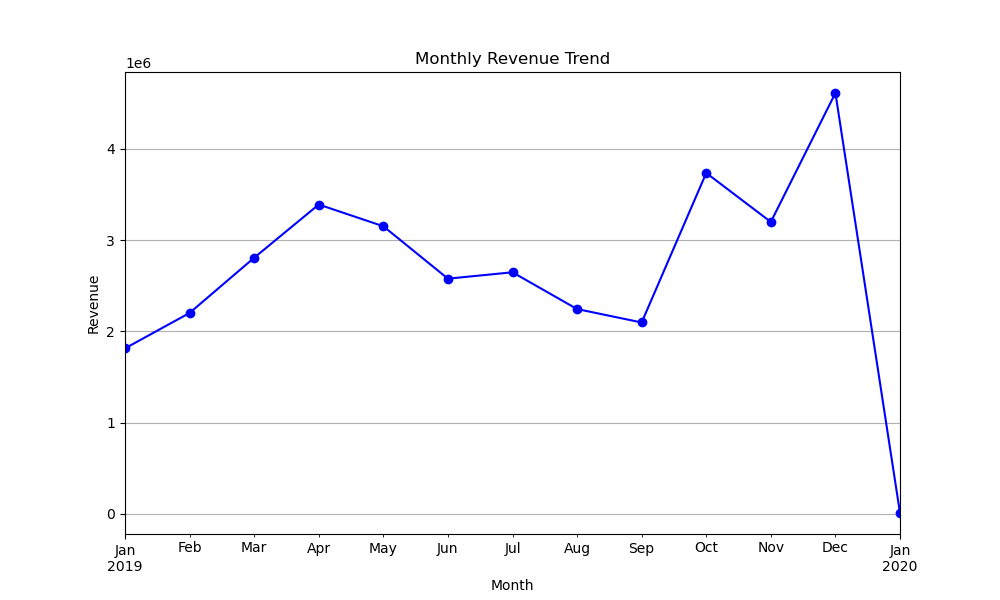
\includegraphics[width=1.0\textwidth]{Lab2/Monthly_Revenue_Trend.png}
    \caption{Monthly Revenue Trend}
    \label{fig:monthly_revenue_trend}
    \vspace{-1em}
\end{figure}


\vspace{-1.5em}
% \subsubsection*{Output}
\begin{figure}[H]
    \centering
    \vspace{2em}
    
    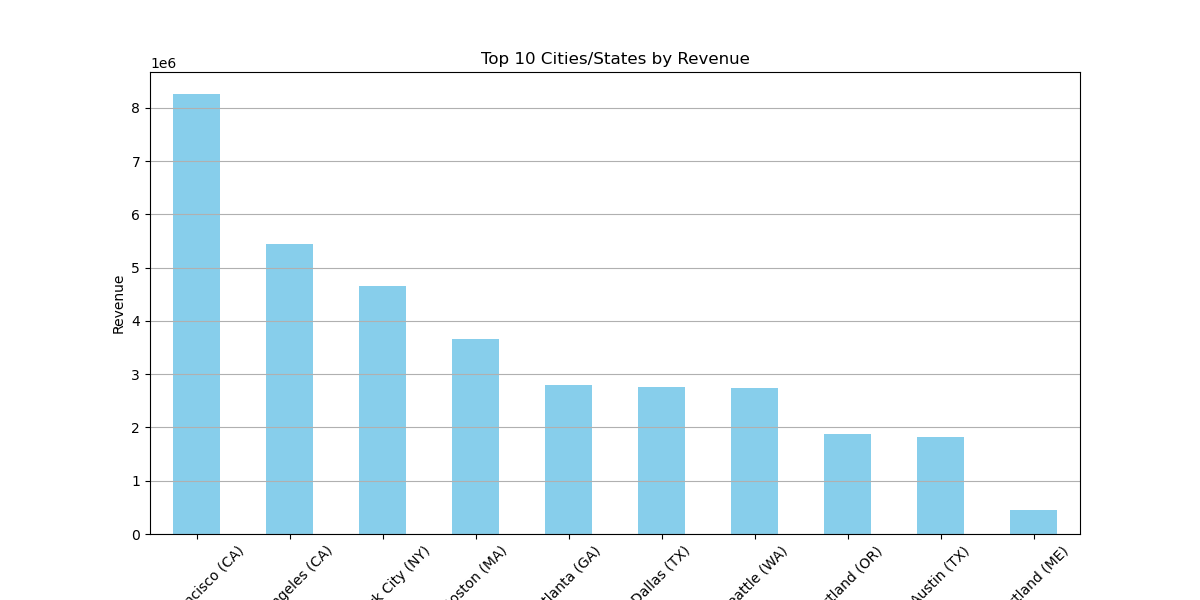
\includegraphics[width=1.0\textwidth]{Lab2/Revenue_by_City.png}
    \caption{Revenue by City/State}
    \label{fig:revenue_by_city_state}
    \vspace{-1em}
\end{figure}


\vspace{-1.5em}
\subsubsection*{Output}
\begin{figure}[H]
    \centering
    \vspace{-2em}
    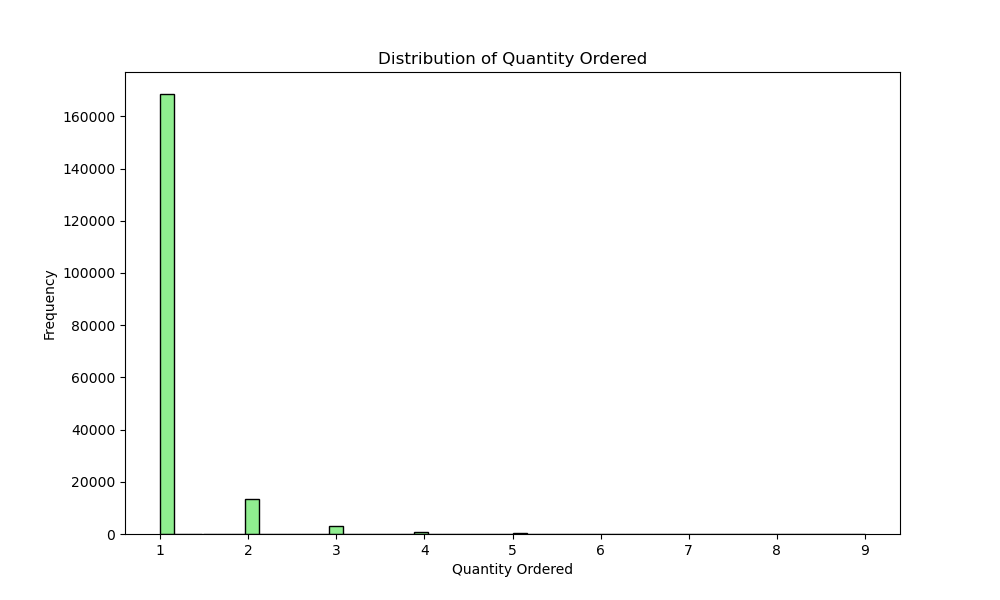
\includegraphics[width=1.0\textwidth]{Lab2/Histogram_Distribution_of_Quality.png}
    \caption{Distribution of Quality}
    \label{fig:distribution_of_quality}
    \vspace{-1em}
\end{figure}


\vspace{-1.5em}
\subsubsection*{Output}
\begin{figure}[H]
    \centering
    \vspace{-2em}
    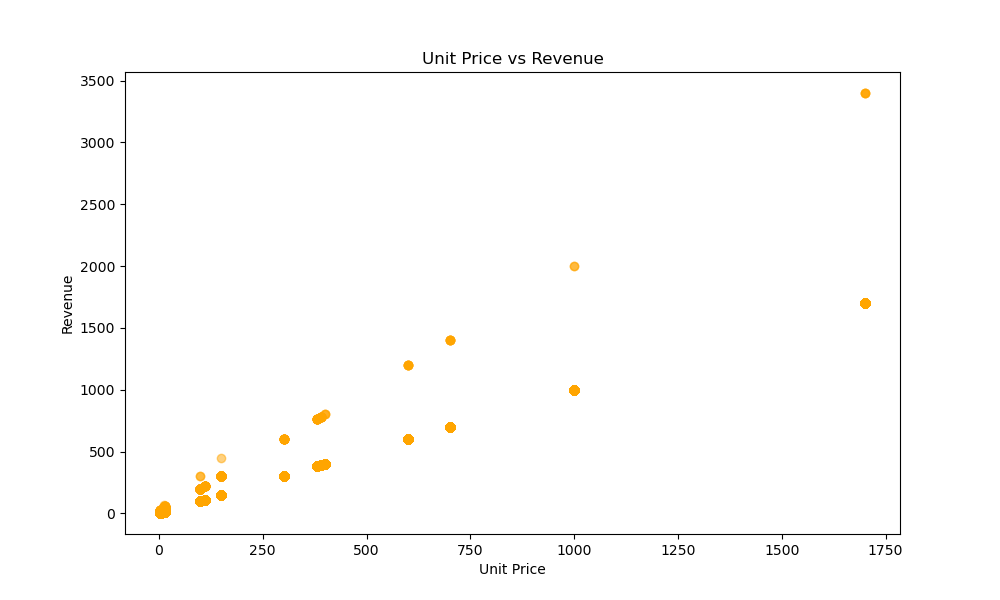
\includegraphics[width=1.0\textwidth]{Lab2/Unit_Price_Vs_Revenue.png}
    \caption{Unit Price vs Revenue}
    \label{fig:unit_price_vs_revenue}
    \vspace{-1em}
\end{figure}


%-----------------------------------------------
% Task 5
%-----------------------------------------------
\subsection{Task 5: Flower Classification Insights (Seaborn Visualization)}


\vspace{-0.1em}
\subsubsection*{Code Implementation}
% \vspace{-1em}
\begin{lstlisting}[style=pythonStyle, caption={}]
# Task 5: Flower Classification Insights (Seaborn Visualization)


import seaborn as sns
import matplotlib.pyplot as plt


iris = sns.load_dataset('iris')
print("First 5 rows of the dataset:")
print(iris.head())


sns.pairplot(iris, hue='species', palette='Set2')
plt.suptitle("Pair Plot of Iris Dataset", y=1.02)
plt.show()

# Step 4: Correlation heatmap of numerical features
correlation = iris.drop('species', axis=1).corr()
plt.figure(figsize=(6,5))
sns.heatmap(correlation, annot=True, cmap='coolwarm')
plt.title("Correlation Heatmap of Numerical Features")
plt.show()

# Step 5: Boxplot of petal length per species
plt.figure(figsize=(6,4))
ax = sns.boxplot(x='species', y='petal_length', data=iris, palette='Set3')
if ax.get_legend():   # remove legend if exists
    ax.get_legend().remove()
plt.title("Boxplot of Petal Length per Species")
plt.show()

# Step 6: Insights based on visualizations
print("\nInsights:")
print("1. Petal length and petal width are highly correlated and clearly separate Iris-setosa from the other species.")
print("2. Boxplot confirms that Iris-setosa has much smaller petal lengths, Iris-versicolor is intermediate, and Iris-virginica has the largest petal lengths, making them good features for classification.")
    
\end{lstlisting}

\vspace{1em} 
% \subsubsection*{Output}
\begin{outputbox}
\begin{verbatim}

    First 5 rows of the dataset:
    
   sepal_length  sepal_width  petal_length  petal_width species
0           5.1          3.5           1.4          0.2  setosa
1           4.9          3.0           1.4          0.2  setosa
2           4.7          3.2           1.3          0.2  setosa
3           4.6          3.1           1.5          0.2  setosa
4           5.0          3.6           1.4          0.2  setosa

\end{verbatim}
\end{outputbox}

% \vspace{-1.5em}
% \subsubsection*{Output}
\begin{figure}[H]
    \centering
    \vspace{-0.1em}
    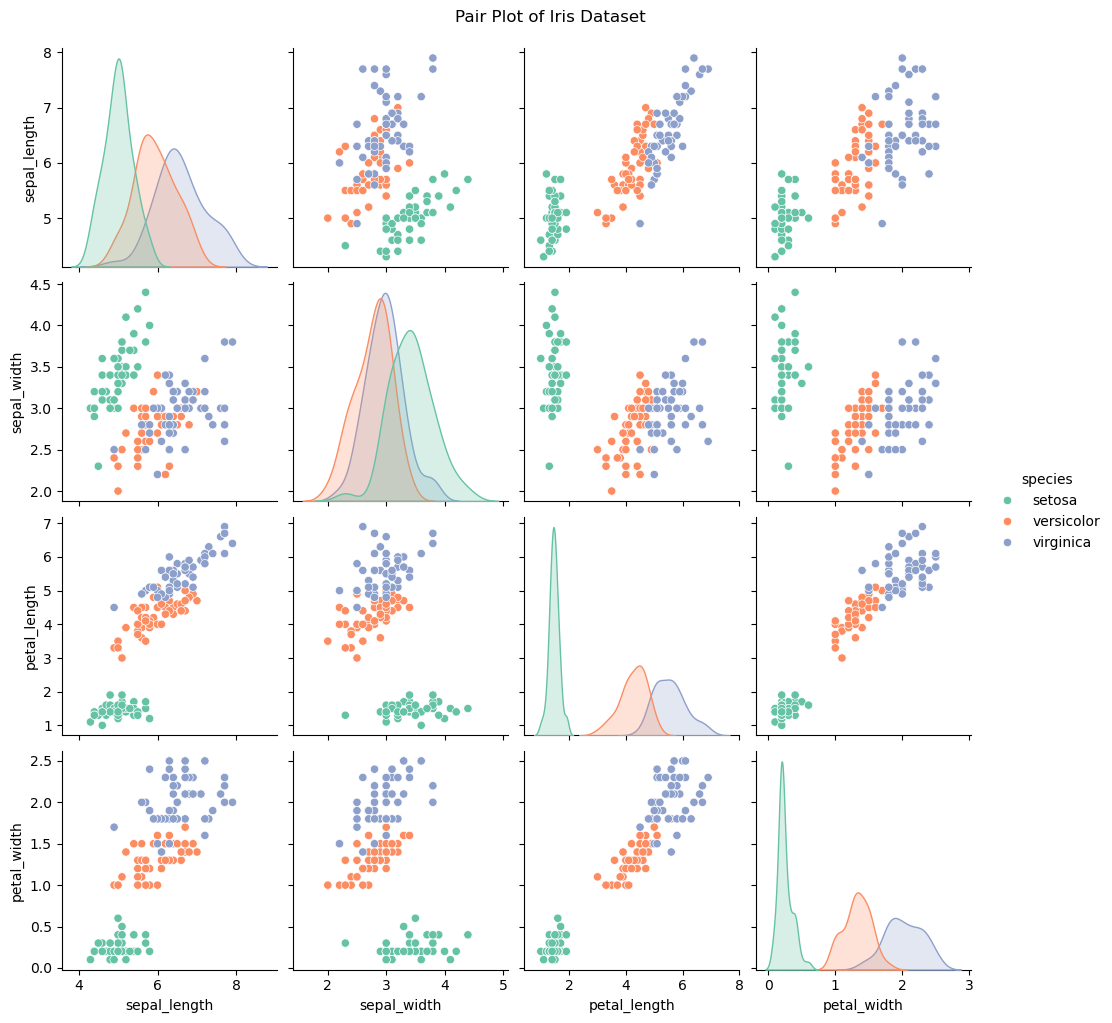
\includegraphics[width=1.0\textwidth]{Lab2/iris_pairplot.png}
    \caption{Pair Plot of Iris Dataset}
    \label{fig:iris_pairplot}
    \vspace{-1em}
\end{figure}

\vspace{-1.5em}
% \subsubsection*{Output}
\begin{figure}[H]
    \centering
    \vspace{-2em}
    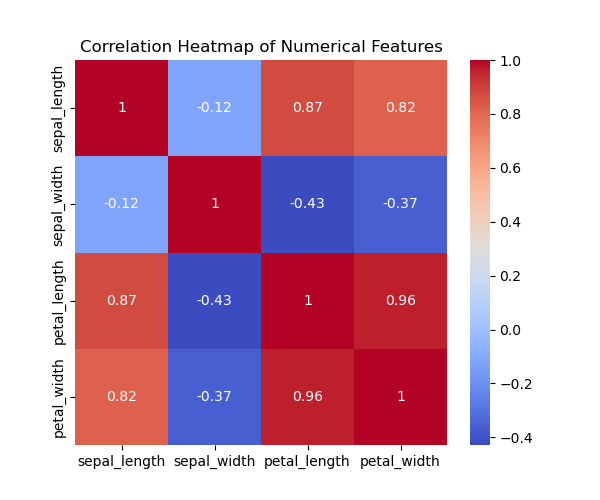
\includegraphics[width=0.9\textwidth]{Lab2/iris_correlation_heatmap.png}
    \caption{Correlation Heatmap of Iris Dataset}
    \label{fig:iris_correlation_heatmap}
    \vspace{-1em}
\end{figure}
% \subsubsection*{Output}
\begin{figure}[H]
    \centering
    \vspace{-0.1em}
    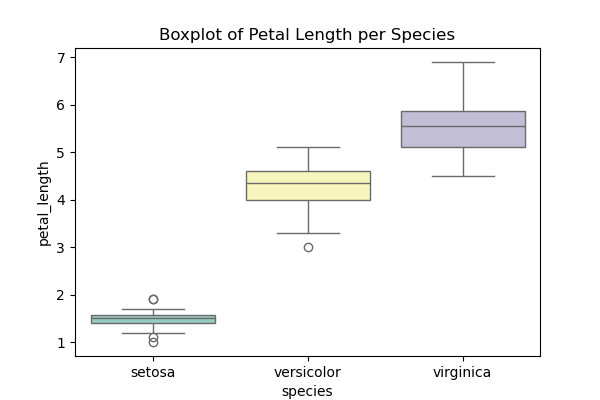
\includegraphics[width=0.9\textwidth]{Lab2/iris_petal_length_boxplot.png}
    \caption{Boxplot of Petal Length per Species}
    \label{fig:iris_petal_length_boxplot}
    \vspace{-1em}
\end{figure}
\begin{outputbox}
\begin{verbatim}
Insights:

1. Petal length and petal width are highly correlated and clearly 
separate Iris-setosa from the other species.

2. Boxplot confirms that Iris-setosa has much smaller petal lengths, 
Iris-versicolor is intermediate, and Iris-virginica has the largest
petal lengths, making them good features for classification.
\end{verbatim}
\end{outputbox}


%-----------------------------------------------
% Project
%-----------------------------------------------
\subsection{Mini Project: Air Quality and Pollution Impact on Health}


\vspace{-0.1em}
\subsubsection*{Code Implementation}
\vspace{-0.1em}
\begin{lstlisting}[style=pythonStyle, caption={}]
# Mini Project: Air Quality & Pollution Impact on Health
# Dataset: AirQualityUCI.csv

# Step 1: Import libraries
import pandas as pd
import numpy as np
import matplotlib.pyplot as plt
import seaborn as sns

# Step 2: Load dataset
data = pd.read_csv('AirQualityUCI.csv', sep=';', decimal=',')  # UCI dataset uses ';' and ','

# Step 3: Inspect dataset
print("First 5 rows:")
print(data.head())
print("\nColumn names:")
print(data.columns)

# Step 4: Keep relevant columns
data = data[['Date', 'Time', 'CO(GT)', 'NOx(GT)', 'PT08.S5(O3)', 'T', 'RH', 'AH']]

# Step 5: Convert Date to datetime
data['Date'] = pd.to_datetime(data['Date'], format='%d/%m/%Y', errors='coerce')

# Step 6: Handle missing values
# Replace -200 values (used in dataset for missing) with NaN
data.replace(-200, np.nan, inplace=True)

# Option 1: Drop rows with missing pollutant values
data_clean = data.dropna(subset=['CO(GT)', 'NOx(GT)', 'PT08.S5(O3)'])

# Step 7: Extract month safely
data_clean = data_clean.copy()  # make a copy to avoid SettingWithCopyWarning
data_clean['Month'] = data_clean['Date'].dt.month
data_clean['Month'] = data_clean['Date'].dt.month

# Step 8: Compute monthly average pollutant levels
monthly_avg = data_clean.groupby('Month')[['CO(GT)', 'NOx(GT)', 'PT08.S5(O3)']].mean()
print("\nMonthly average pollutant levels:")
print(monthly_avg)

# Step 9: Visualize pollution trends
plt.figure(figsize=(10,5))
sns.lineplot(data=monthly_avg, marker='o')
plt.title("Monthly Average Pollutant Levels")
plt.xlabel("Month")
plt.ylabel("Average Concentration")
plt.xticks(range(1,13))
plt.legend(['CO', 'NOx', 'O3'])
plt.grid(True)
plt.show()

# Bar plot
monthly_avg.plot(kind='bar', figsize=(10,6))
plt.title("Monthly Average Pollutant Levels")
plt.xlabel("Month")
plt.ylabel("Average Concentration")
plt.show()

# Step 10: Correlation between pollutants and temperature
corr_matrix = data_clean[['CO(GT)', 'NOx(GT)', 'PT08.S5(O3)', 'T']].corr()
print("\nCorrelation matrix:")
print(corr_matrix)

# Visualize correlation
plt.figure(figsize=(6,5))
sns.heatmap(corr_matrix, annot=True, cmap='coolwarm')
plt.title("Correlation between Pollutants and Temperature")
plt.show()

# Step 11: Research insights (examples)
print("\nResearch Insights:")
print("1. NOx levels tend to spike during winter months (lower temperatures).")
print("2. O3 (ozone) levels show positive correlation with temperature, higher in warmer months.")
   
\end{lstlisting}

\vspace{1em} 
\subsubsection*{Output}
\begin{Numbox}
\begin{verbatim}

First 5 rows:

         Date      Time  CO(GT)  PT08.S1(CO)  NMHC(GT)  C6H6(GT)  \
0  10/03/2004  18.00.00     2.6       1360.0     150.0      11.9   
1  10/03/2004  19.00.00     2.0       1292.0     112.0       9.4   
2  10/03/2004  20.00.00     2.2       1402.0      88.0       9.0   
3  10/03/2004  21.00.00     2.2       1376.0      80.0       9.2   
4  10/03/2004  22.00.00     1.6       1272.0      51.0       6.5   

   PT08.S2(NMHC)  NOx(GT)  PT08.S3(NOx)  NO2(GT)  PT08.S4(NO2)  PT08.S5(O3)  \
0         1046.0    166.0        1056.0    113.0        1692.0       1268.0   
1          955.0    103.0        1174.0     92.0        1559.0        972.0   
2          939.0    131.0        1140.0    114.0        1555.0       1074.0   
3          948.0    172.0        1092.0    122.0        1584.0       1203.0   
4          836.0    131.0        1205.0    116.0        1490.0       1110.0   

      T    RH      AH  Unnamed: 15  Unnamed: 16  
0  13.6  48.9  0.7578          NaN          NaN  
1  13.3  47.7  0.7255          NaN          NaN  
2  11.9  54.0  0.7502          NaN          NaN  
3  11.0  60.0  0.7867          NaN          NaN  
4  11.2  59.6  0.7888          NaN          NaN  

Column names:

Index(['Date', 'Time', 'CO(GT)', 'PT08.S1(CO)', 'NMHC(GT)', 'C6H6(GT)',
       'PT08.S2(NMHC)', 'NOx(GT)', 'PT08.S3(NOx)', 'NO2(GT)', 'PT08.S4(NO2)',
       'PT08.S5(O3)', 'T', 'RH', 'AH', 'Unnamed: 15', 'Unnamed: 16'],
      dtype='object')

Monthly average pollutant levels:

         CO(GT)     NOx(GT)  PT08.S5(O3)
Month                                   
1      2.148480  369.077703  1149.868243
2      2.019608  308.499109  1041.827094
3      2.175063  247.727811  1081.532544
4      2.180712  146.885768   978.977528
5      1.986819  126.813708   958.008787
6      1.969002  129.225919   962.033275
7      1.832276  129.970149  1007.791045
8      1.279951   70.596577   775.545232
9      2.335227  282.422727  1078.315909
10     2.807487  345.350267  1258.243316
11     2.760502  427.708464  1195.838558
12     2.632402  384.532588  1150.579143

\end{verbatim}
\end{Numbox}

\begin{figure}[H]
    \centering
    \vspace{-0.1em}
    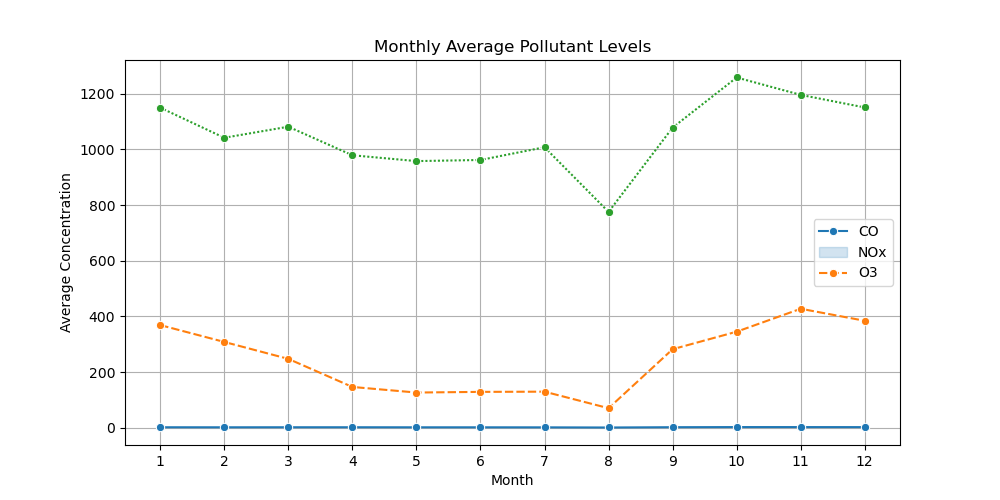
\includegraphics[width=1.0\textwidth]{Lab2/monthly_avg_pollutants_lineplot.png}
    \caption{Monthly Average Pollutant Levels (Line Plot)}
    \label{fig:monthly_avg_pollutants_lineplot}
    % \vspace{-1em}
    \end{figure}

\begin{figure}[H]
    \centering
    \vspace{-0.1em}
    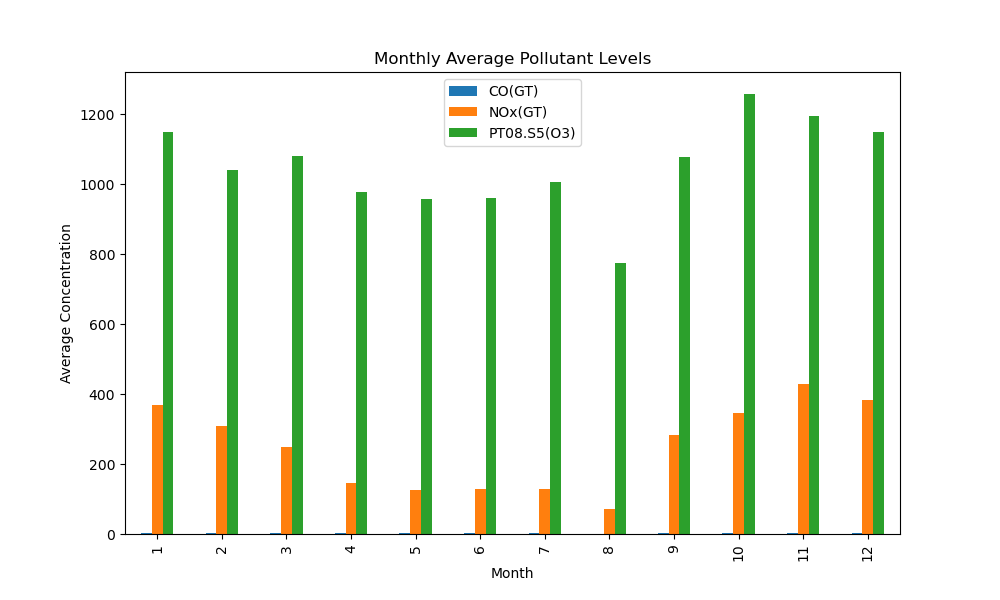
\includegraphics[width=0.7\textwidth]{Lab2/monthly_avg_pollutants_barplot.png}
    \caption{Boxplot of Monthly Average Pollutant Levels}
    \label{fig:monthly_avg_pollutants_barplot}
    % \vspace{-1em}
\end{figure}

\begin{Numbox}
\begin{verbatim}
Correlation matrix:
               CO(GT)   NOx(GT)  PT08.S5(O3)         T
CO(GT)       1.000000  0.786401     0.853474  0.018331
NOx(GT)      0.786401  1.000000     0.788500 -0.276150
PT08.S5(O3)  0.853474  0.788500     1.000000 -0.046148
T            0.018331 -0.276150    -0.046148  1.000000
\end{verbatim}
\end{Numbox}

\begin{figure}[H]
    \centering
    \vspace{-0.1em}
    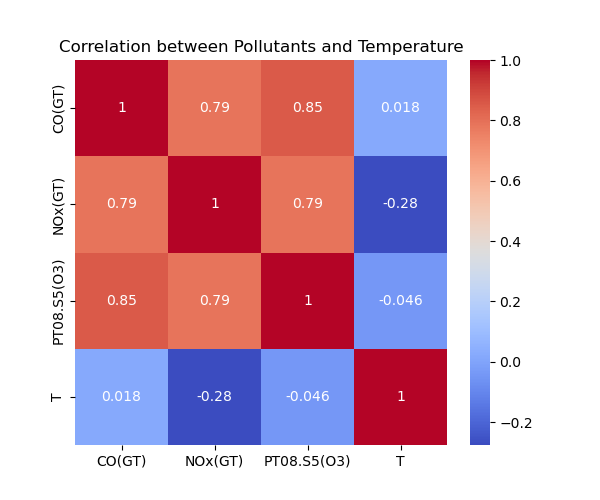
\includegraphics[width=0.7\textwidth]{Lab2/pollutants_temperature_correlation_heatmap.png}
    \caption{Heatmap of Pollutants and Temperature Correlation}
    \label{fig:pollutants_temperature_correlation_heatmap}
    \vspace{-1em}
\end{figure}

\begin{Numbox}
\begin{verbatim}


\end{verbatim}
\end{Numbox}
%-----------------------------------------------
% End of Assignment 2
%-----------------------------------------------


